\subsection{Sequence Diagram}

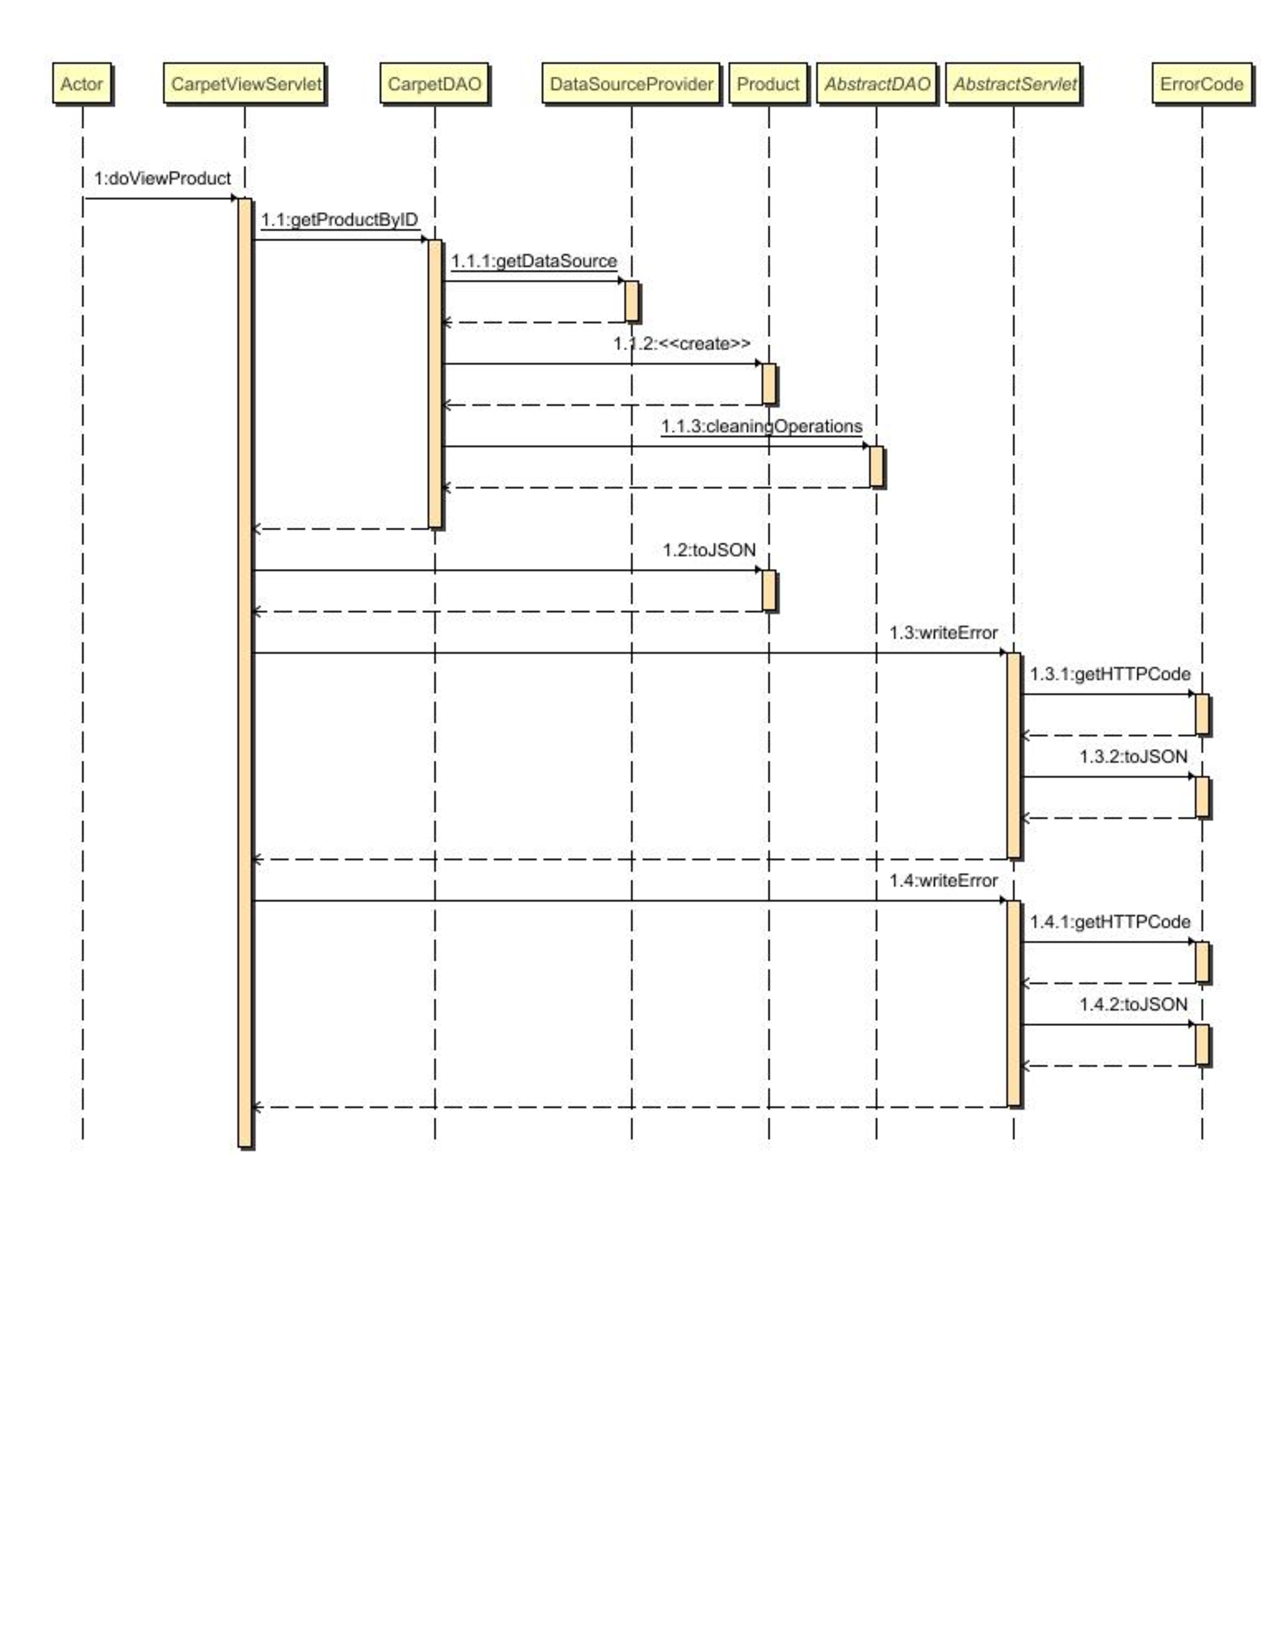
\includegraphics[width=\textwidth]{wab-homework1/sections/BLL/sequenceDiagram1.pdf}

\newpage

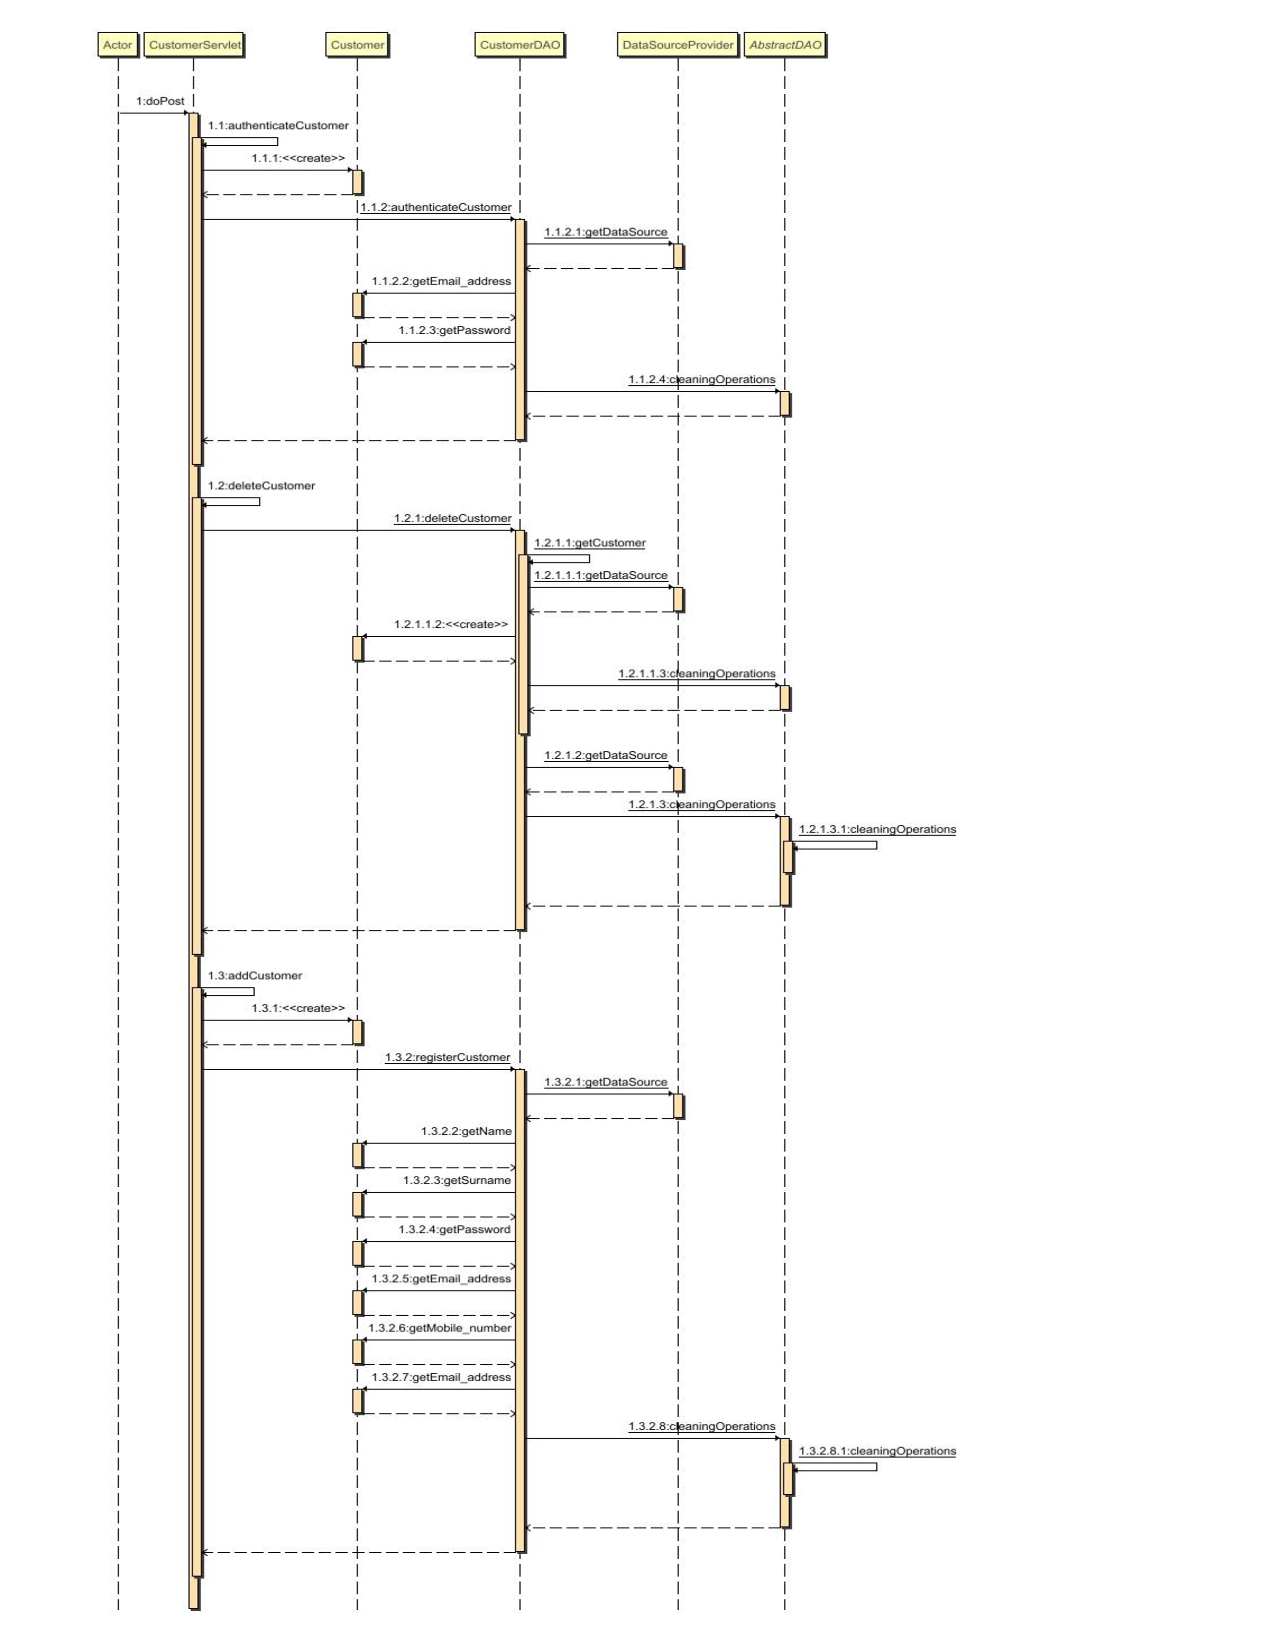
\includegraphics[width=\textwidth]{wab-homework1/sections/BLL/sequenceDiagram2.pdf}

This section presents the sequence diagram for the customer operations performed through the CustomerServlet and CustomerDAO. The login process begins when the customer clicks on the login section and sends a GET request to the CustomerServlet at the URI "customer/login".\\
Subsequently, when the customer enters their email and password and clicks the login button, the data is sent to the servlet via a POST request. The doPost method of the CustomerServlet is then invoked, receiving the HttpServletRequest and HttpServletResponse as parameters.\\
The control flow is then transferred to the CustomerDAO, which receives the connection as an argument and contacts the Database Server to execute an SQL statement to validate the email and password. If any errors occur, control is returned to the SessionServlet, and a new Message object is generated. \\
If the email and password are correct, the customer is directed to the dashboard. Otherwise, an error message indicating an incorrect username or password is displayed, and the customer is redirected accordingly.\\
\\
The registration process begins when the customer clicks on the registration section, and a form with input arguments about the customer appears. After filling out the required data and clicking the submit button, the URI "customer/register" is sent to the CustomerServlet via a POST request. \\
The doPost method of the CustomerServlet is invoked, receiving the HttpServletRequest and HttpServletResponse as parameters. The control flow is then transferred to the CustomerDAO, which receives the connection as an argument and contacts the Database Server to execute an SQL statement to add\\
the data while performing validation checks. If any errors occur, control is returned to the SessionServlet, and a new Message object is generated. If the defined response value is 0, it indicates that the registration was successful, and the customer is directed to the dashboard. Otherwise,\\ 
an error message indicating the issue is displayed, and the customer is redirected accordingly.\\
In addition to the login and registration processes, the CustomerServlet and CustomerDAO also facilitate the update process for the customer. The update process begins when the customer clicks on the update section and sends a GET request to the CustomerServlet at the URI "customer/update".\\
The CustomerServlet retrieves the customer's current information from the Database Server using the CustomerDAO and populates the form with the retrieved data. Once the customer has made the desired changes and clicked the submit button, a POST request is sent to the CustomerServlet at the URI "customer/update". \\
The doPost method of the CustomerServlet is then invoked, receiving the HttpServletRequest and HttpServletResponse as parameters. The control flow is then transferred to the CustomerDAO, which receives the connection as an argument and contacts the Database Server to execute an SQL statement to update the customer's information while performing validation checks. \\
If any errors occur, control is returned to the SessionServlet, and a new Message object is generated. If the update is successful, the customer is directed to the dashboard. Otherwise, an error message indicating the issue is displayed, and the customer is redirected accordingly.\\

\newpage